\documentclass[12pt]{beamer}

%%%%%%%%%%%%%%%%%%% Theme

\usetheme{metropolis}

%%%%%%%%%%%%%%%%%%% Packages

\usepackage[french, english]{babel}
\usepackage{packages/sleek-beamer}

%%%%%%%%%%%%%%%%%%% Bibliography

\addbibresource{./resources/bib/references.bib}

%%%%%%%%%%%%%%%%%%% Titlepage

\title{Renewable Energy Production Forecast}
\subtitle{PROJ0016 - Big Data Project}
\author{Yann Claes, Gaspard Lambrechts and François Rozet}
\institute{University of Liège}
\date{\today}
\titlelogo{./resources/pdf/logo.pdf}
\framelogo{./resources/pdf/logo.pdf}

%%%%%%%%%%%%%%%%%%%

\DeclareSIUnit\voltampere{VA}

%%%%%%%%%%%%%%%%%%%

\begin{document}

\maketitle

\section{Photovoltaic production}

\begin{frame}{Extension of the panel-wise model}
    Required inputs to the model:
    \begin{itemize}
        \item Time series
        \item Latitude and longitude of each panel
        \item Area of each panel
        \item Surface azimuth
    \end{itemize}
\end{frame}

\begin{frame}{Extension of the panel-wise model}
    Nice-to-have inputs:
    \begin{itemize}
        \item Panel efficiency $\eta$
        \item Panel tilt $\beta$
    \end{itemize}
    If not possible to obtain, we could investigate the use of PyStan.
\end{frame}

\begin{frame}{Provincial model - Naive example}
    Sample example for the naive model $P = \eta I A$
    \begin{figure}
        \centering
        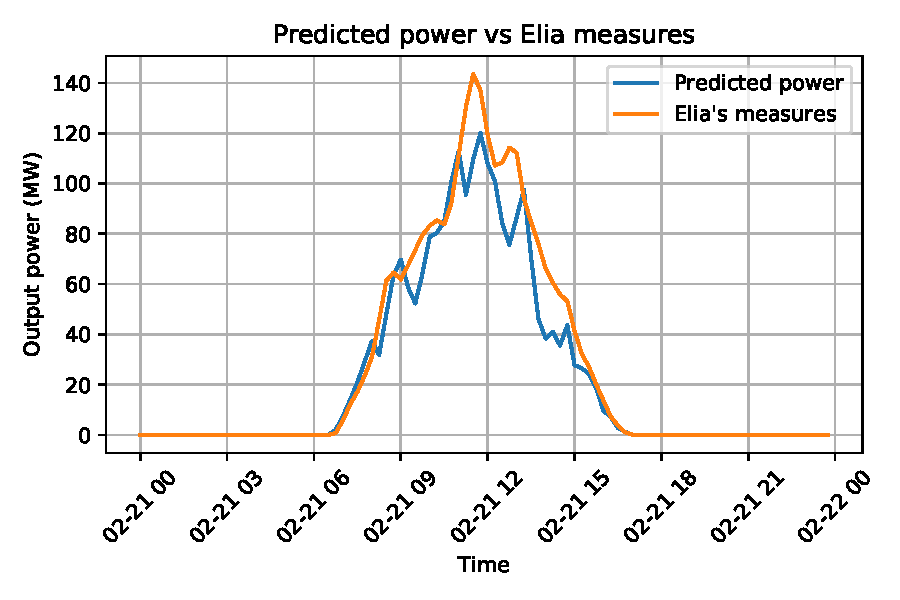
\includegraphics[width=.8\textwidth]{resources/pdf/province_example.pdf}
        \noskipcaption{Naive physical model example.}
        \label{fig:province_example}
    \end{figure}
\end{frame}

\begin{frame}{Provincial model - Improvements}
    To improve this naive model, implement a PyStan model to define uncertainties on:
    \begin{itemize}
        \item The efficiency $\eta$
        \item The irradiance measures $I$
        \item The provincial panel area $A$
    \end{itemize}
\end{frame}

\begin{frame}{Provincial model - Posterior example}
    \begin{itemize}
        \item Fit on period ranging from the 15\up{th} of February 2019 to the 23\up{rd} (excluded)
        \item Predict for the 23\up{rd}
    \end{itemize}
    The predictive model is defined as a normal distribution centered around
	$\mu = \eta I A$ with a standard deviation $\sigma = \SI{100}{\kilo\watt}$.
\end{frame}

\begin{frame}{Provincial model - Posterior example}
	\begin{figure}
	    \centering
	    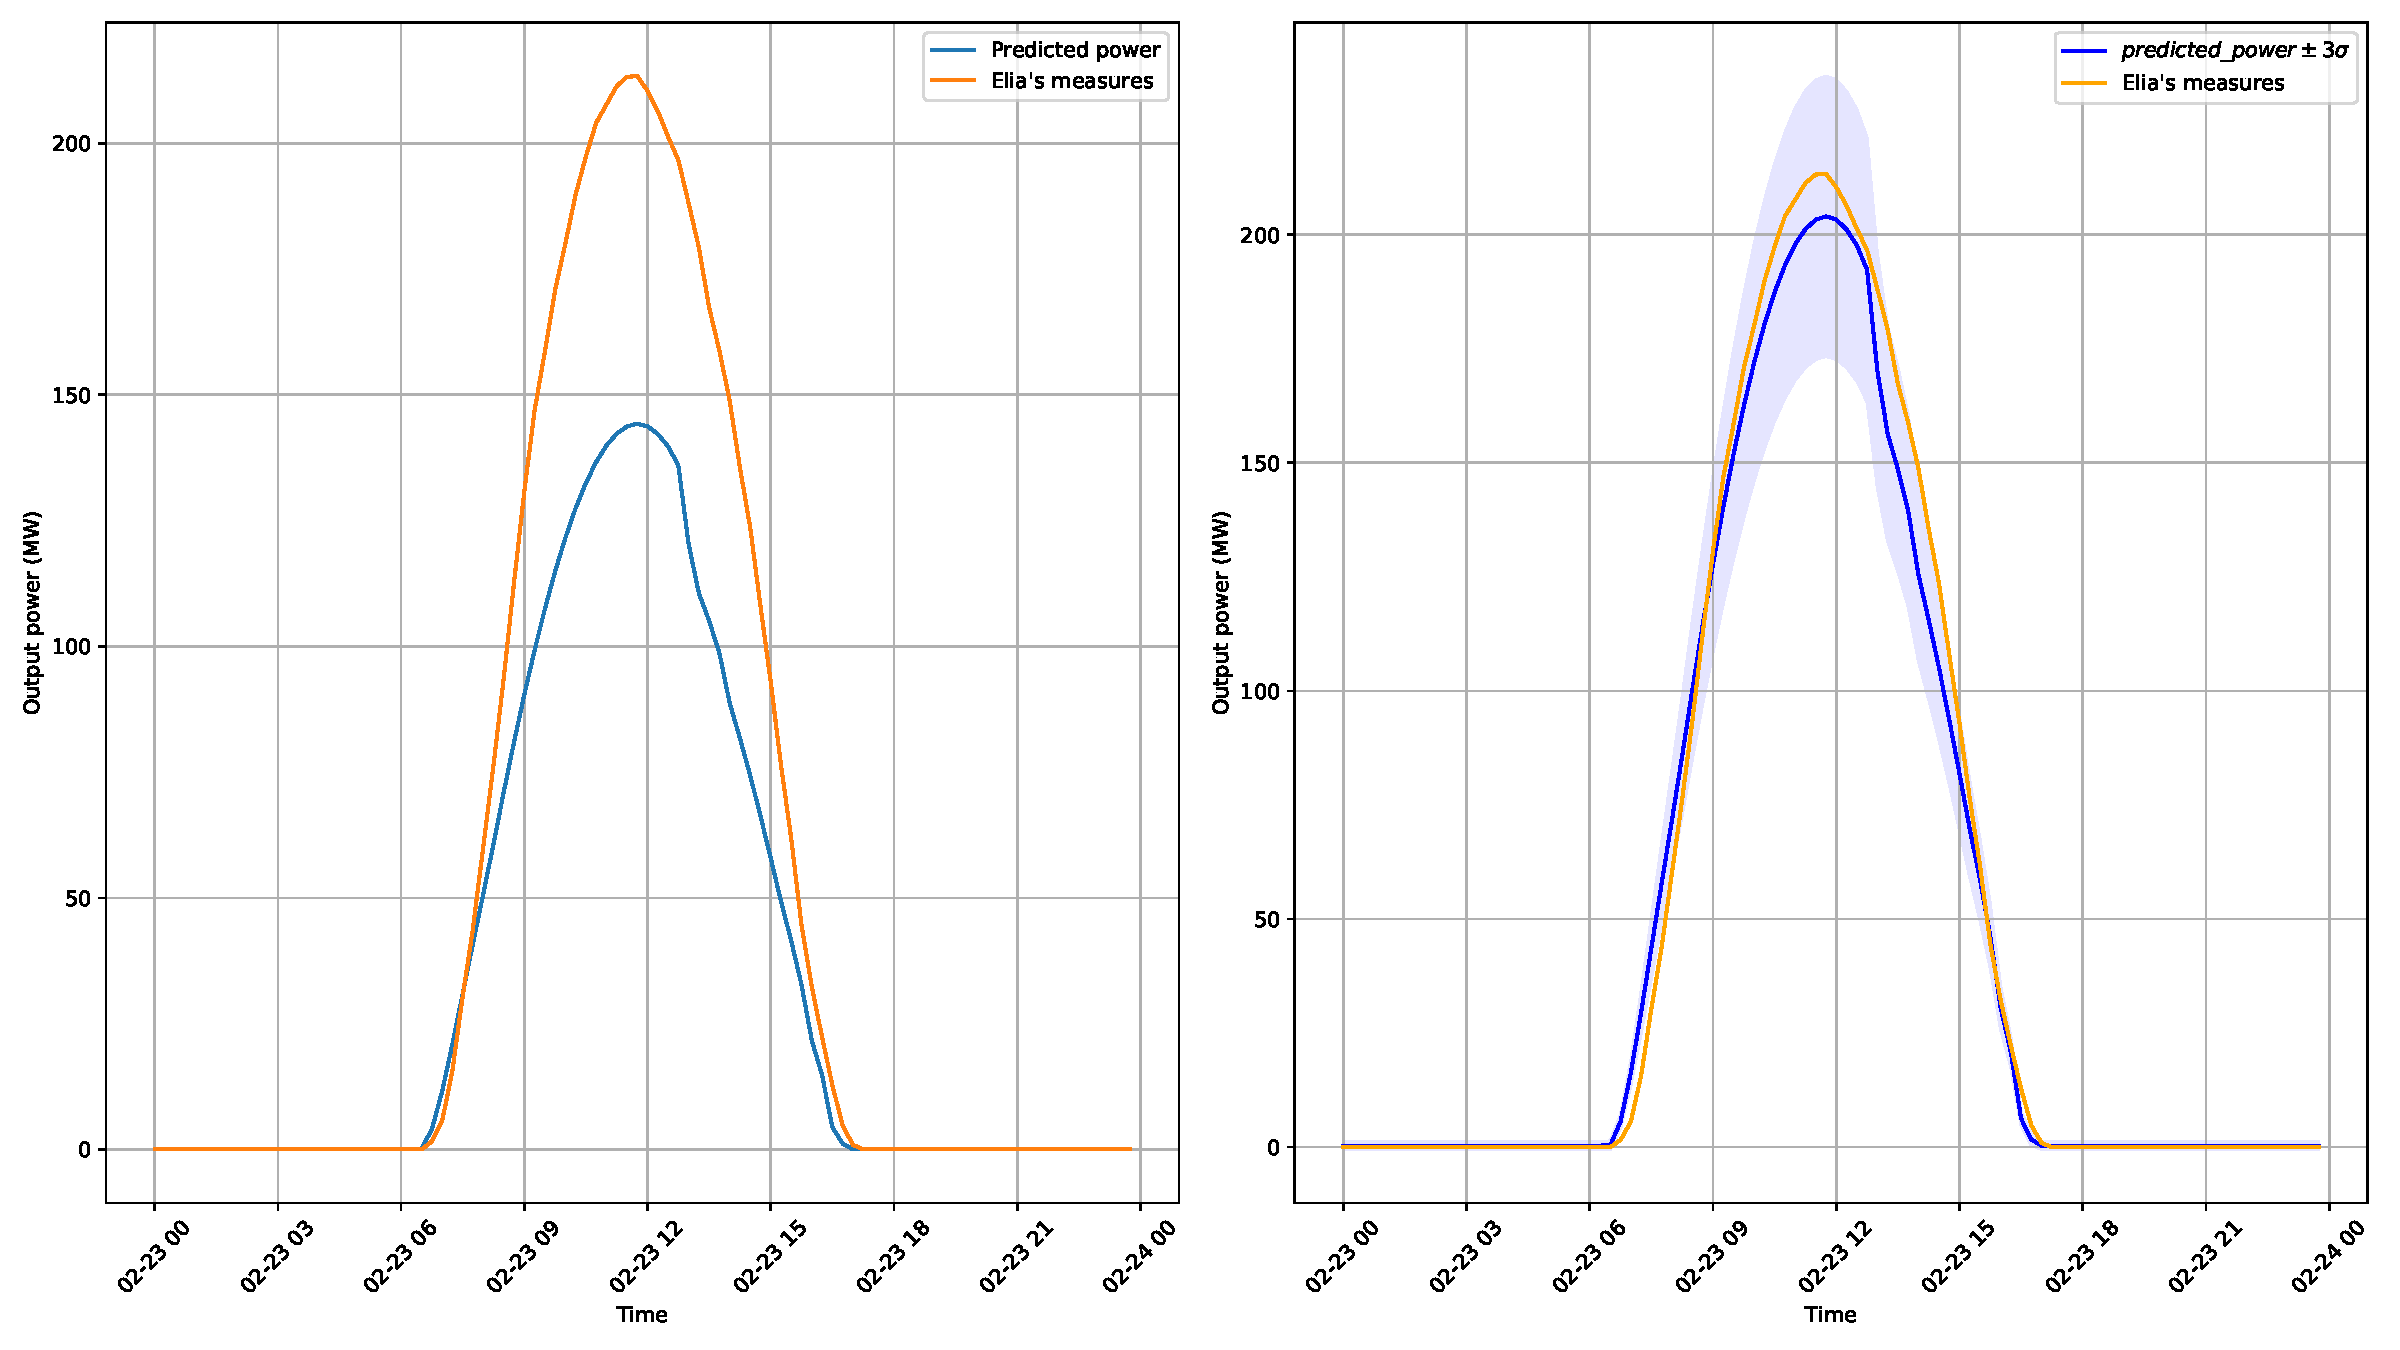
\includegraphics[width=.85\textwidth]{resources/pdf/comparison_naive_post.pdf}
	    \noskipcaption{Comparison between prior and posterior predictive models.}
	    \label{fig:comparison_naive_post}
	\end{figure}
\end{frame}

\begin{frame}{Provincial model - Posterior example}
	\begin{figure}
	    \centering
	    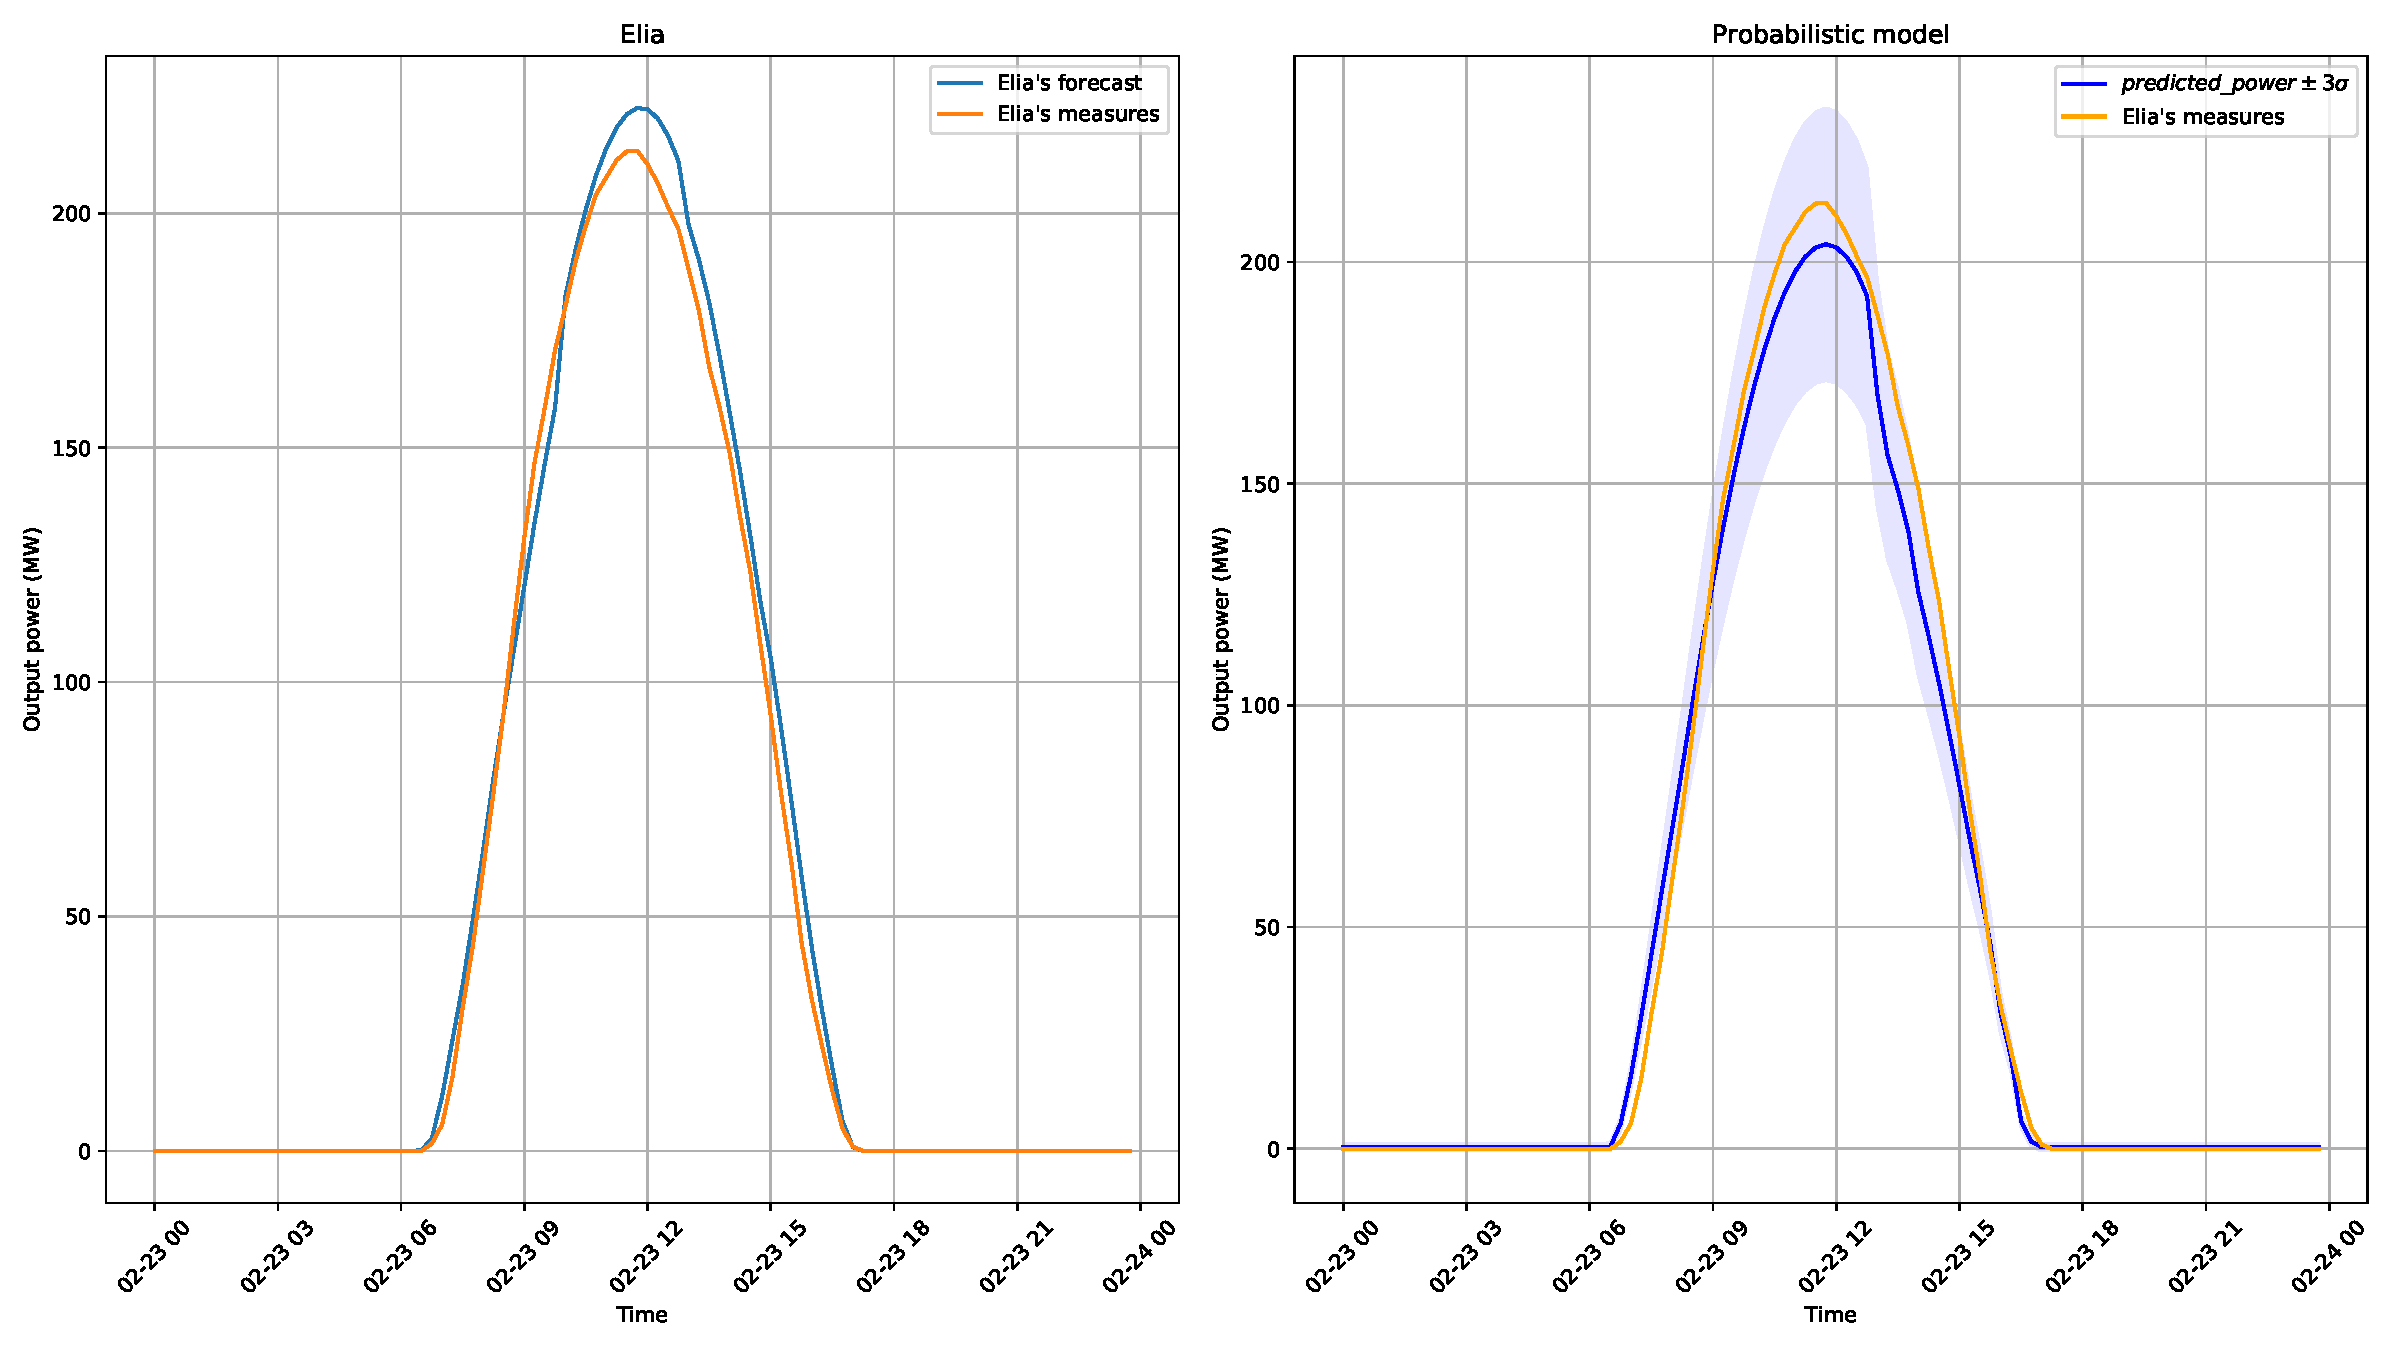
\includegraphics[width=.85\textwidth]{resources/pdf/comparison_elia_post.pdf}
	    \noskipcaption{Comparison between Elia's forecast and the posterior model.}
	    \label{fig:comparison_elia_post}
	\end{figure}
\end{frame}

\begin{frame}{Provincial model - Posterior example}
	\begin{table}
    	\centering
        \begin{tabular}{l|l|l}
                  & MSE      & RMSE   \\ \hline
        Elia      & 84.988 & 9.219    \\ \hline
        Naive     & 2211.522 & 47.027 \\ \hline
        Posterior & 126.439  & 11.244
        \end{tabular}
        \noskipcaption{MSE and RMSE for all three models \cite{bocquet}.}
        \label{tab:elia_post}
    \end{table}
\end{frame}

\begin{frame}{Provincial model - Conclusions?}
    Same methodology for 15\up{th} of March 2019 to the 23\up{rd}.
    \begin{figure}
        \centering
        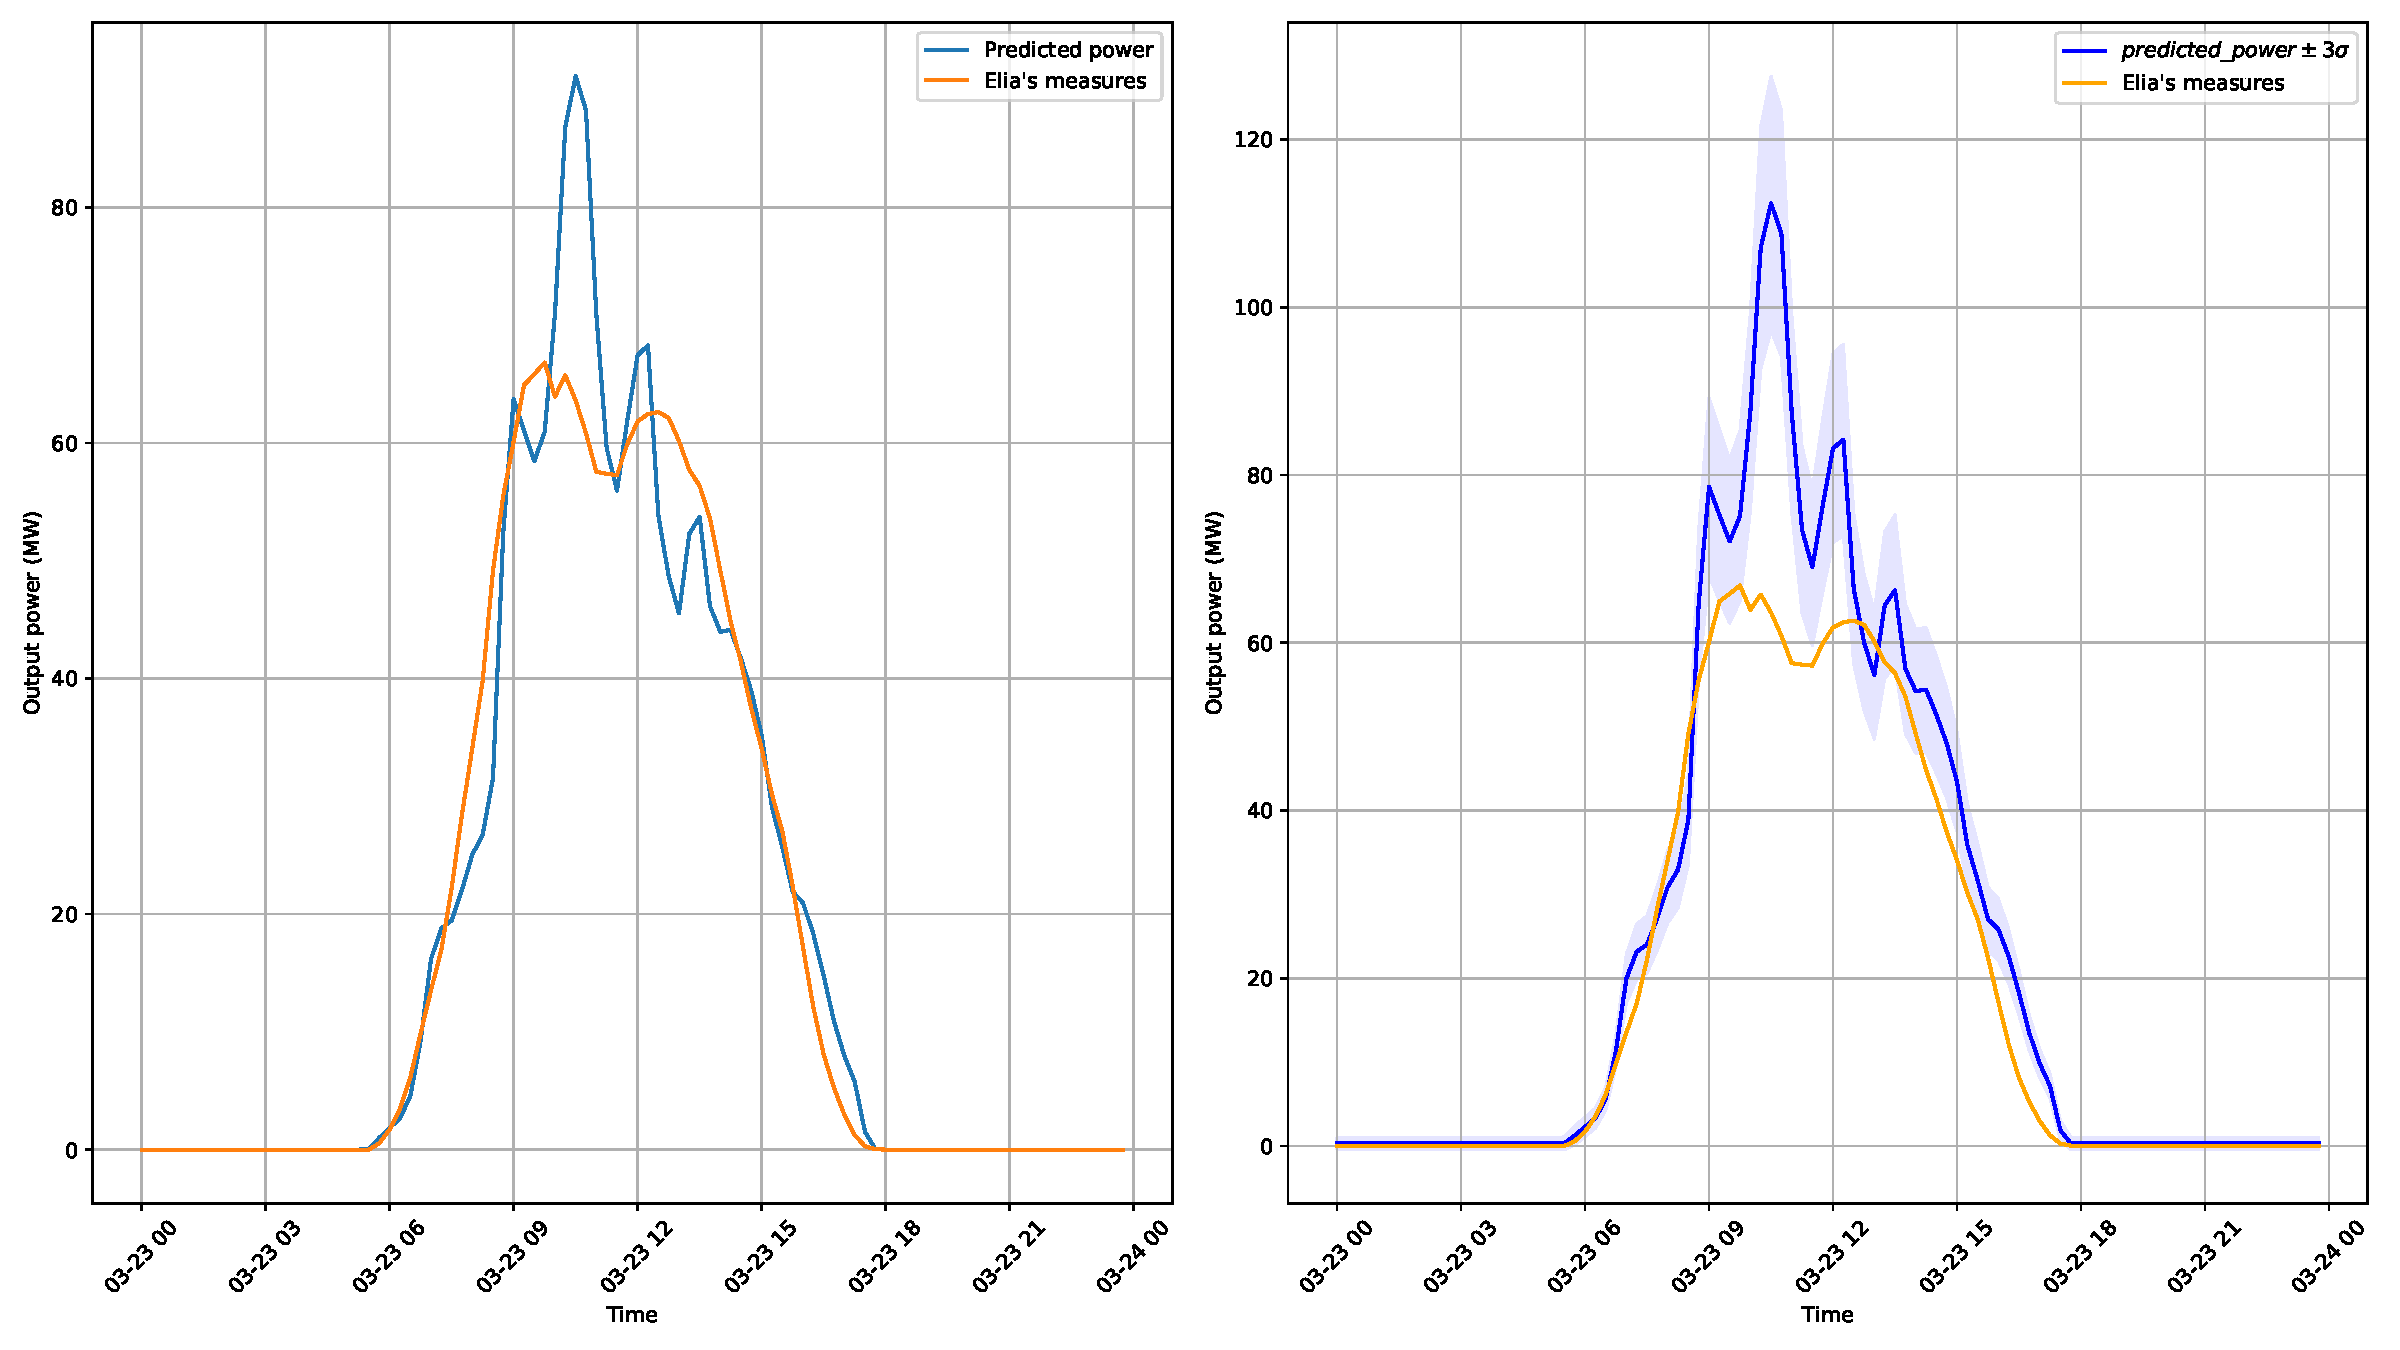
\includegraphics[width=.85\textwidth]{resources/pdf/bad_naive_post.pdf}
        \noskipcaption{Same example for March 2019 (naive vs posterior model).}
        \label{fig:bad_naive_post}
    \end{figure}
\end{frame}

\begin{frame}{Provincial model - Conclusions ?}
    \begin{figure}
        \centering
        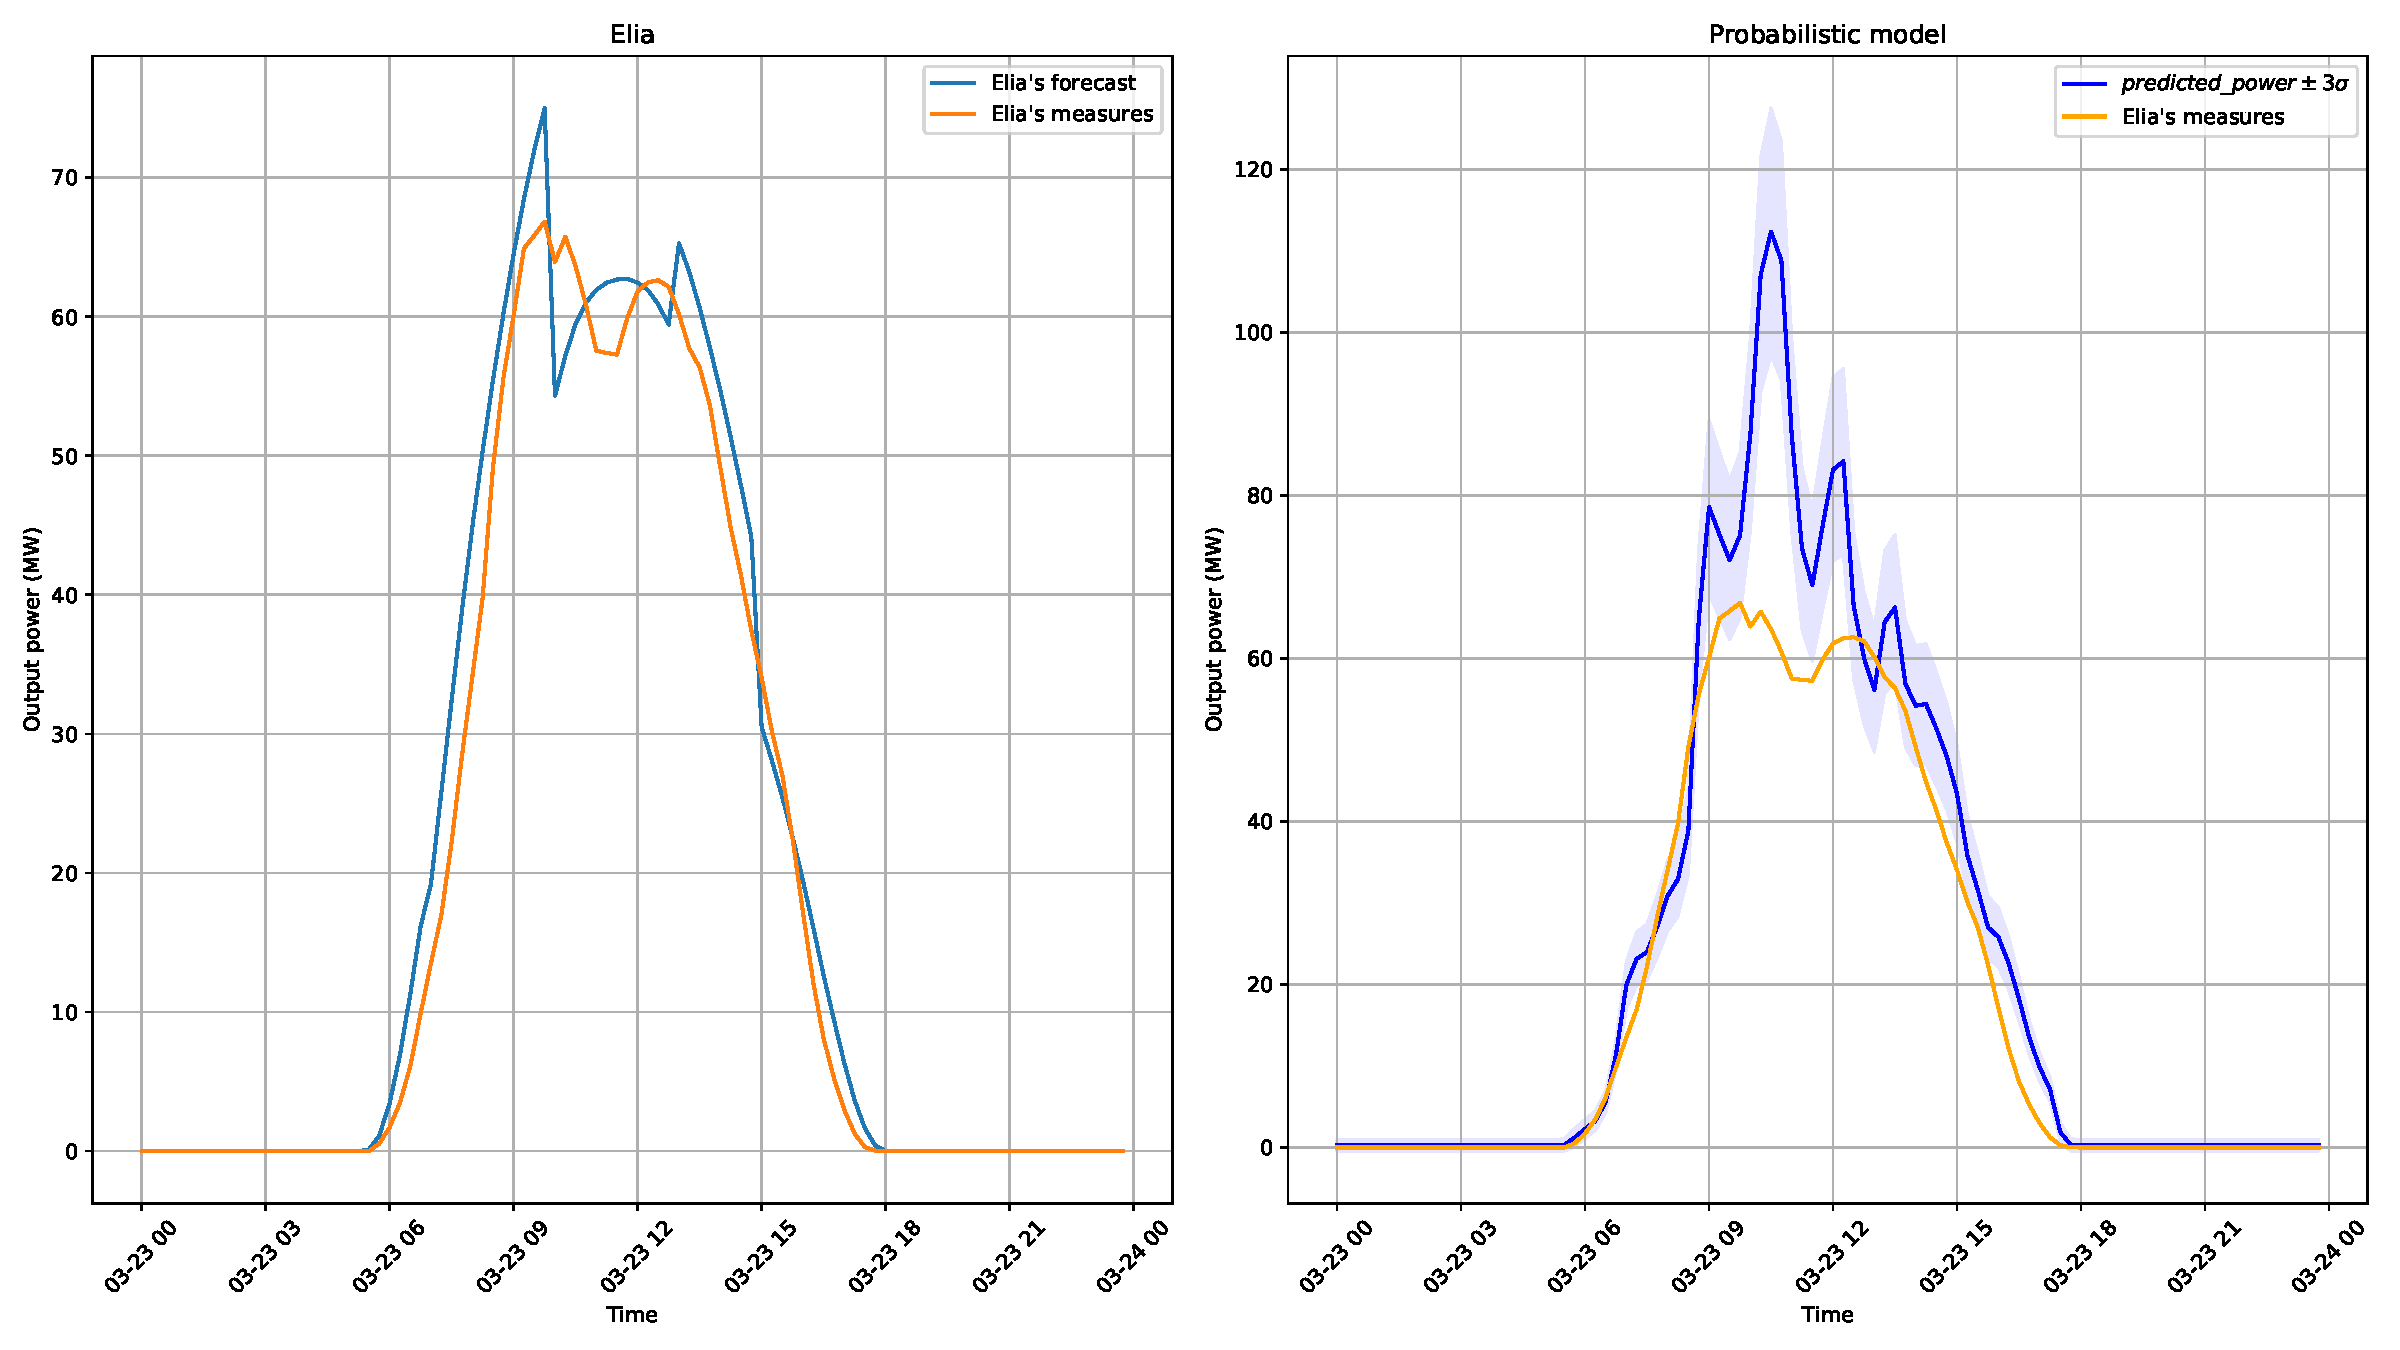
\includegraphics[width=.9\textwidth]{resources/pdf/bad_elia_post.pdf}
        \noskipcaption{Same example for March 2019 (Elia vs posterior model).}
        \label{fig:bad_elia_post}
    \end{figure}
\end{frame}

\begin{frame}{Next objectives}
Two main aspects need to be completed:
\begin{itemize}
    \item Finding a (reliable) historical-forecast API
    \item Complete the analysis of the provincial model (baseline models, representative period)
\end{itemize}
\end{frame}
\section{Photovoltaic panels enumeration}

\begin{frame}{Reminder}
    We have a \alert{suitable dataset} : a large collection of annotated high resolution aerial imagery.
    
    Our goal for this review was to \alert{design and/or train} a neural network able to \alert{detect} photovoltaic panels in satellite images, hence the name \emph{Automatic Detection Of Photovoltaic Panels Through Remote Sensing}\footnote{Inspired from the paper \og{}Automatic Detection of Solar Photovoltaic Arrays in High Resolution Aerial Imagery\fg{} \cite{malof2016automatic}.} or \alert{ADOPPTRS}\footnote{Repository : \texttt{\href{https://github.com/francois-rozet/adopptrs}{https://github.com/francois-rozet/adopptrs}}}.
\end{frame}

\begin{frame}{DeepSolar}
    Since our goal are very similar, we looked after \alert{DeepSolar} \cite{yu2018deepsolar} model.
    
    \begin{figure}
        \centering
        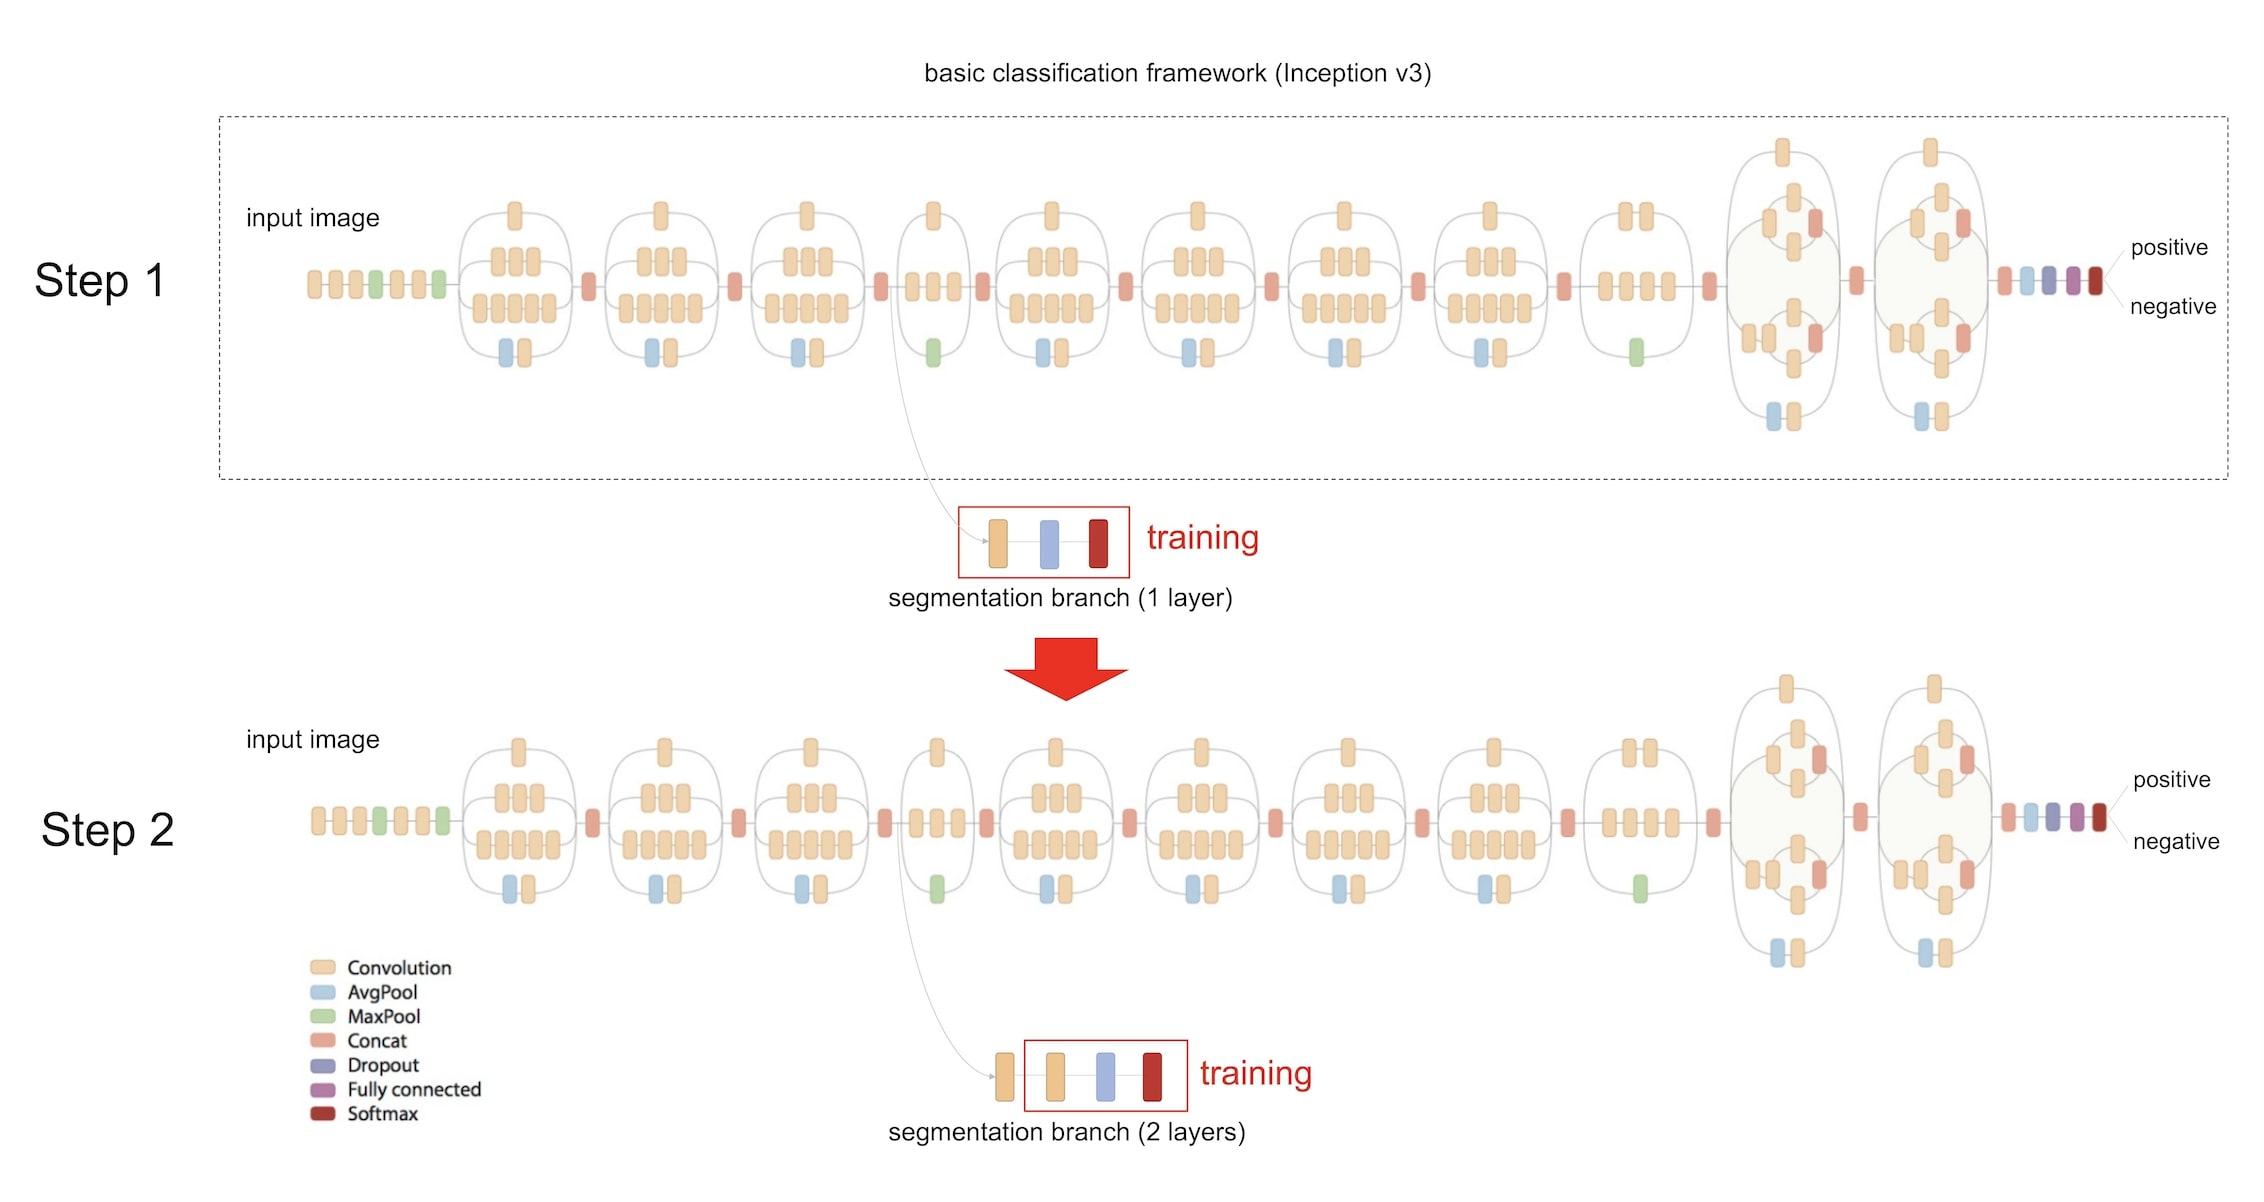
\includegraphics[width=0.9\textwidth]{resources/jpg/cnn_arch.jpg}
        \caption{DeepSolar's network representation. \cite{yu2018deepsolar}}
    \end{figure}

\end{frame}

\begin{frame}{DeepSolar}
    Fairly complicated.  It incorporates \alert{both} image classification (Google Inception V3 \cite{szegedy2016rethinking}) and semantic segmentation in a single convolutional neural network.
    
    Classification branch is used to localize the panels. The segmentation branch is used to estimate their size.
    
    We believe that reproducing such network is not within our capabilities.
\end{frame}

\begin{frame}{U-Net}
    One of the most famous segmentation model is U-Net \cite{ronneberger2015u}.
    
    \begin{figure}
        \centering
        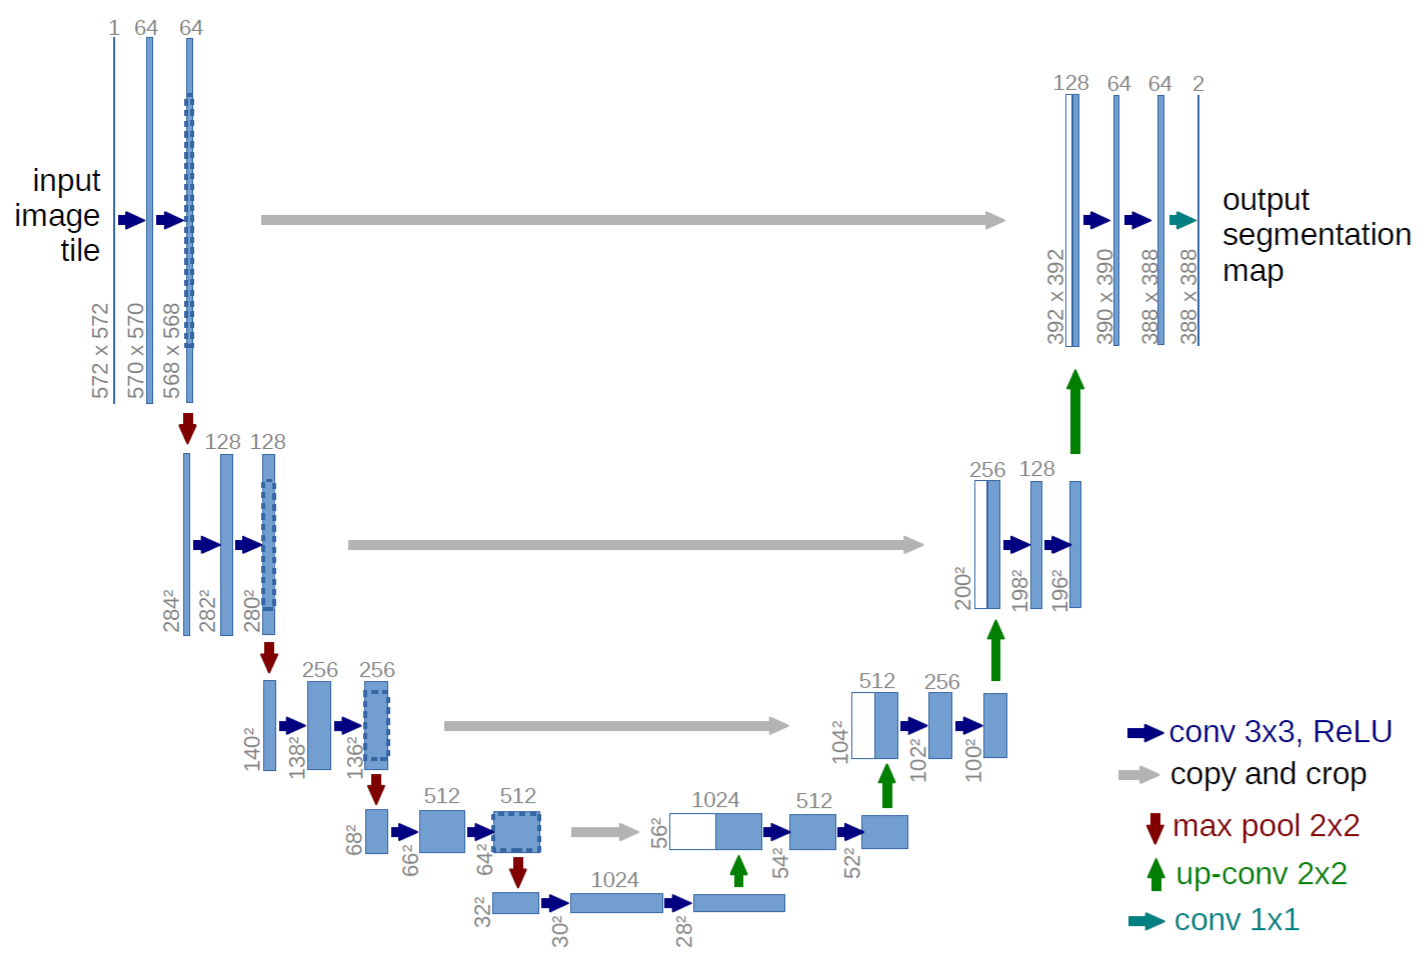
\includegraphics[width=0.8\textwidth]{resources/png/unet.png}
        \caption{U-net architecture. \cite{ronneberger2015u}}
    \end{figure}
\end{frame}

\begin{frame}{U-Net}
    Initially designed for biomedical image segmentation, it actually works very well for a lot of applications and is \alert{easy to train} thanks to the \alert{pass-through} mechanism preventing vanishing gradients.

    We have implemented U-Net using \texttt{PyTorch}.
\end{frame}

\begin{frame}{Training}
    We divided our dataset in 3 subsets :
    \begin{enumerate}
        \item A training set (\SI{75}{\percent}) for training the models
        \item A validation set (\SI{12.5}{\percent}) for selecting the best model(s)
        \item A testing set (\SI{12.5}{\percent}) to evaluate our final model(s)
    \end{enumerate}
\end{frame}

\begin{frame}{Training - Loss}
    We looked after a \emph{loss function for imbalanced segmentation} and found the \alert{dice coefficient} and \alert{intersection over union}.
    
    \begin{align*}
        IoU(A, B) & = \frac{\abs{A \cap B}}{\abs{A \cup B}} & Dice(A, B) & = \frac{2 \abs{A \cap B}}{\abs{A} + \abs{B}}
    \end{align*}
    
    Both are similar, but we chose to implement \alert{dice}.
\end{frame}

\begin{frame}{Training - Loss}
    \begin{figure}
        \centering
        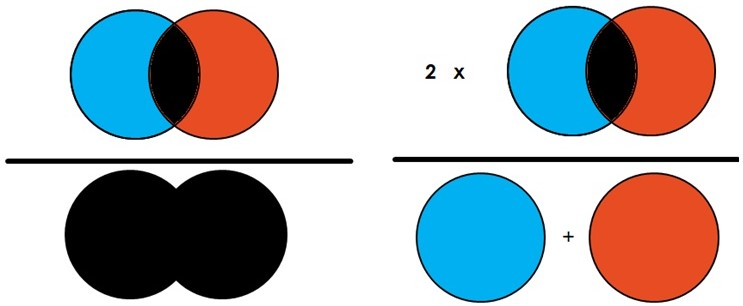
\includegraphics[width=\textwidth]{resources/jpg/iou_dice.jpg}
        \caption{Illustration of Intersection over Union (left) and Dice Coefficient (right). \cite{towardsdatascience}}
    \end{figure}
\end{frame}

\begin{frame}{Training - Data augmentation}
    Our approach to data augmentation is to randomly apply some transformation(s) \alert{while training}. At each epoch, the training set is slightly different.
    
    \visible<2->{
    \begin{itemize}
        \item Rotations : \SI{90}{\degree}, \SI{180}{\degree}, \SI{270}{\degree} 
        \item Flipping horizontally or vertically
        \item Brightness alteration
        \item Saturation alteration
        \item Contrast alteration
    \end{itemize}
    }
\end{frame}

\begin{frame}{Training - Data augmentation}
    \begin{figure}
        \centering
        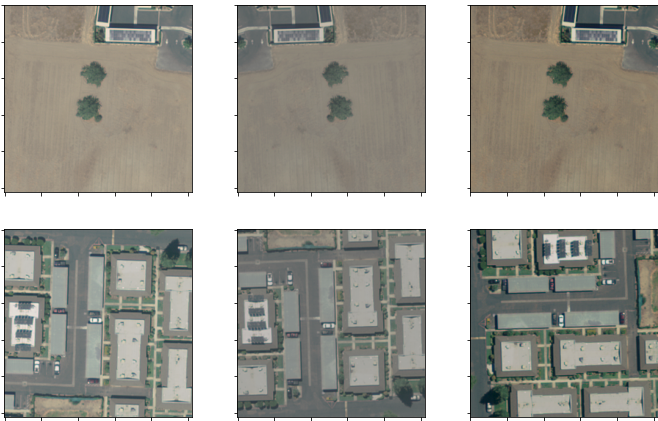
\includegraphics[width=\textwidth]{resources/png/augmentation_crop.png}
        \caption{Some images transformations.}
    \end{figure}
\end{frame}

\begin{frame}{Results}
    For now, our best model achieves an average \alert{dice loss} ($1 - dice$) of \SI{26.5}{\percent} on the validation set. But the \alert{confusion matrix} is more informative :
    
    \begin{table}
        \centering
        \begin{tabular}{cc|cc}
            && \multicolumn{2}{c}{Truth} \\
            && 0 & 1 \\ \hline
            \multirow{2}{*}{Prediction} & 0 & \num{3.236e5} & \num{1.054e3} \\
            & 1 & \num{3.096e2} & \num{2.690e3} \\
        \end{tabular}
        \noskipcaption{Average confusion matrix on the validation set.}
        \label{tab:confusion_matrix}
    \end{table}
\end{frame}

\begin{frame}{Results}
    \begin{align*}
        accuracy & = \frac{TP + TN}{TP + TN + FP + FN} =  \SI{99.58}{\percent} \\
        precision & = \frac{TP}{TP + FP} = \SI{89.69}{\percent} \\
        recall & = \frac{TP}{TP + FN} = \SI{71.92}{\percent}
    \end{align*}
    
    Our model rarely classifies something else as a photovoltaic panel but it often fails to recognize a photovoltaic panel\footnote{Accuracy isn't relevant because of class imbalance}.
\end{frame}

\begin{frame}{Samples}
    \begin{figure}
        \centering
        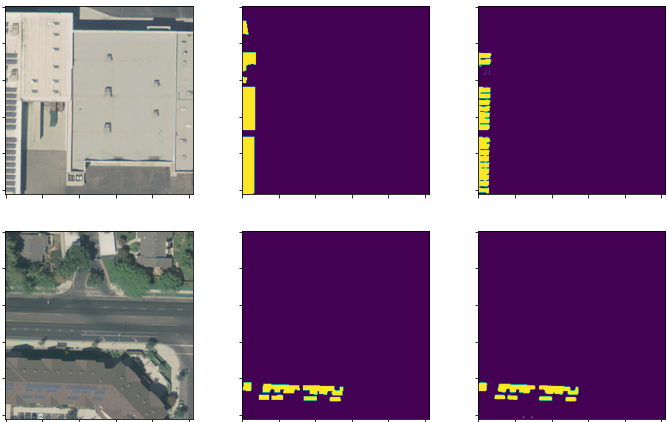
\includegraphics[width=\textwidth]{resources/png/representative_0_crop.png}
        \caption{Representative behavior}
    \end{figure}
\end{frame}

\begin{frame}{Samples}
    \begin{figure}
        \centering
        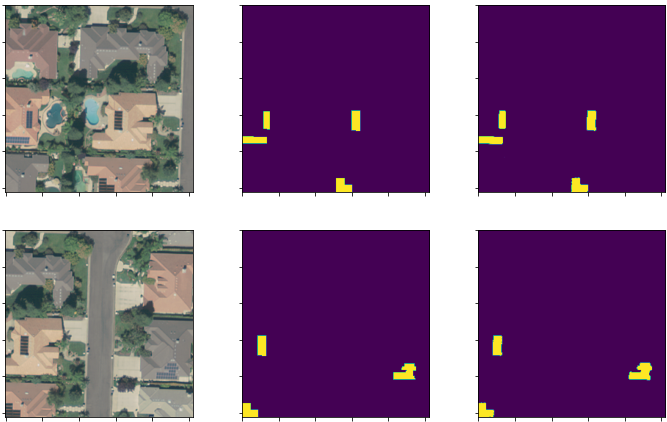
\includegraphics[width=\textwidth]{resources/png/representative_1_crop.png}
        \caption{Representative behavior}
    \end{figure}
\end{frame}

\begin{frame}{Samples}
    \begin{figure}
        \centering
        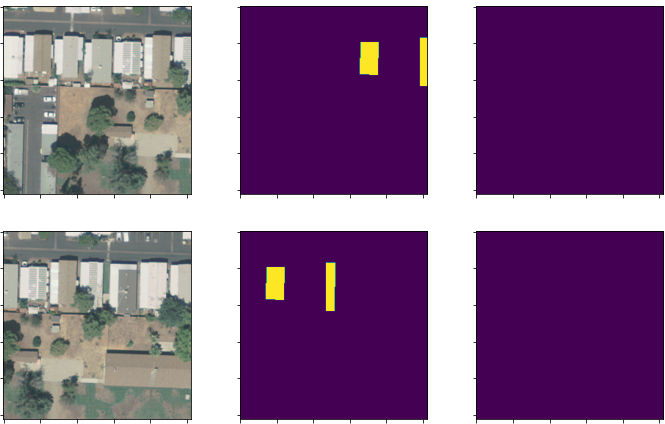
\includegraphics[width=\textwidth]{resources/png/bad_color_crop.png}
        \caption{Abnormal panel color}
    \end{figure}
\end{frame}

\begin{frame}{Samples}
    \begin{figure}
        \centering
        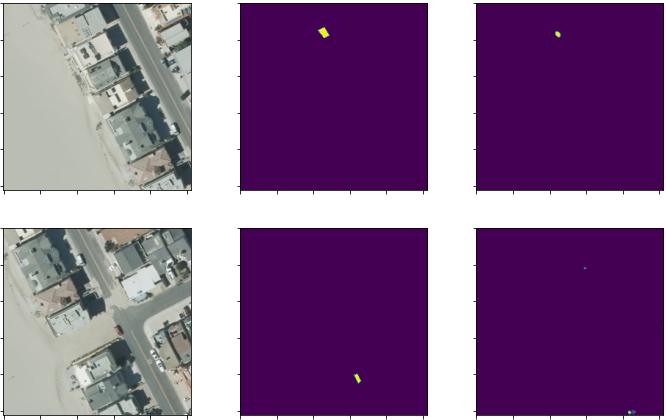
\includegraphics[width=\textwidth]{resources/png/bad_size_crop.png}
        \caption{Abnormal panel size}
    \end{figure}
\end{frame}

\begin{frame}{Samples}
    \begin{figure}
        \centering
        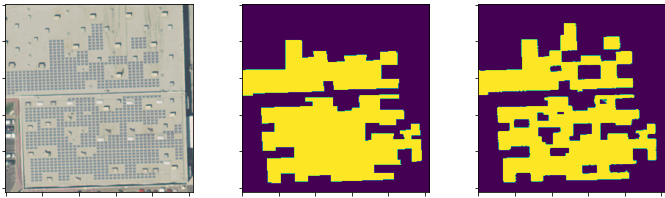
\includegraphics[width=\textwidth]{resources/png/beter_than_annotation_crop.png}
        \caption{Predictions better than annotations}
    \end{figure}
    Such \emph{inaccurate} annotations could be one of the causes of the relatively bad \alert{recall} of our model.
\end{frame}

\begin{frame}{Next objectives}
    \begin{itemize}
        \item We still want to improve our model and try a few others before applying it to the detection in Liège.
        \item There is still to do a few post-processing to convert our predictions into usable photovoltaic panel locations.
    \end{itemize}
\end{frame}

\section{Wind production}

\begin{frame}{Classification of wind forecasting problems\footnote{Wang et. al, A Review of Wind Power Forecasting Models, 2011 \cite{wang2011windpower}}}
    \begin{itemize}
        \item Very-short-term or immediate-short-term (a few hours ahead)
        \item \alert<2->{Short-term (few hours to several days)}
        \item Long-term (multiple days ahead)
    \end{itemize}
    
\end{frame}

\begin{frame}{Classification of forecasting techniques\footnote{Sweeney et. al, The Future of Forecasting for Renewable Energy, 2019 \cite{sweeney2019future}}}
    \begin{enumerate}
        \item \textbf{Physical modeling}: based on Numerical Weather Prediction (NWP)
        \item \alert<2->{\textbf{Statistical modeling}}
            \begin{enumerate}
                \item On the very short term: \emph{time series based forecasting}: the NWP data is not used, only the power time series is used to make the prediction.
                \item On the longer term: \alert<2->{\emph{post processing of NPW}}: the temporal aspect is not considered
            \end{enumerate}
        \item \textbf{Hybrid method}: uses \emph{post processing of NPW} \textbf{and} \emph{of physical modeling}
    \end{enumerate}
\end{frame}

\begin{frame}{Possible improvements on physical model}
    \begin{itemize}
        \item Take hub height wind into account using the log wind profile: $$u(z_2) = u(z_1) \frac{\ln(z_2/z_0)}{\ln(z_1/z_0)}$$
        \item Model in a simple way the self-wake effects according to the wind speed and direction
    \end{itemize}
\end{frame}

\begin{frame}{Statistical model: \alert{\emph{weather to power}}}
    The inputs of our model are (for \num{15} different locations): \resizebox{\textwidth}{!}{
        \begin{tabular}{|c|c|c|c|c|c|c|}
            \hline
            \texttt{windSpeed} & \texttt{windGust} & \texttt{windBearing} & \texttt{temperature} & \texttt{humidity} & \texttt{pressure} & \texttt{airDensity} \\ \hline
            \SI{}{\meter\per{\second}} & \SI{}{\meter\per{\second}} &\alert{\SI{}{\deg}} & \SI{}{\kelvin} & \SI{}{\percent} & \SI{}{\pascal} & \SI{}{\kilogram\per{\meter\cubed}} \\ \hline
        \end{tabular}
    }
    \begin{figure}
        \centering
        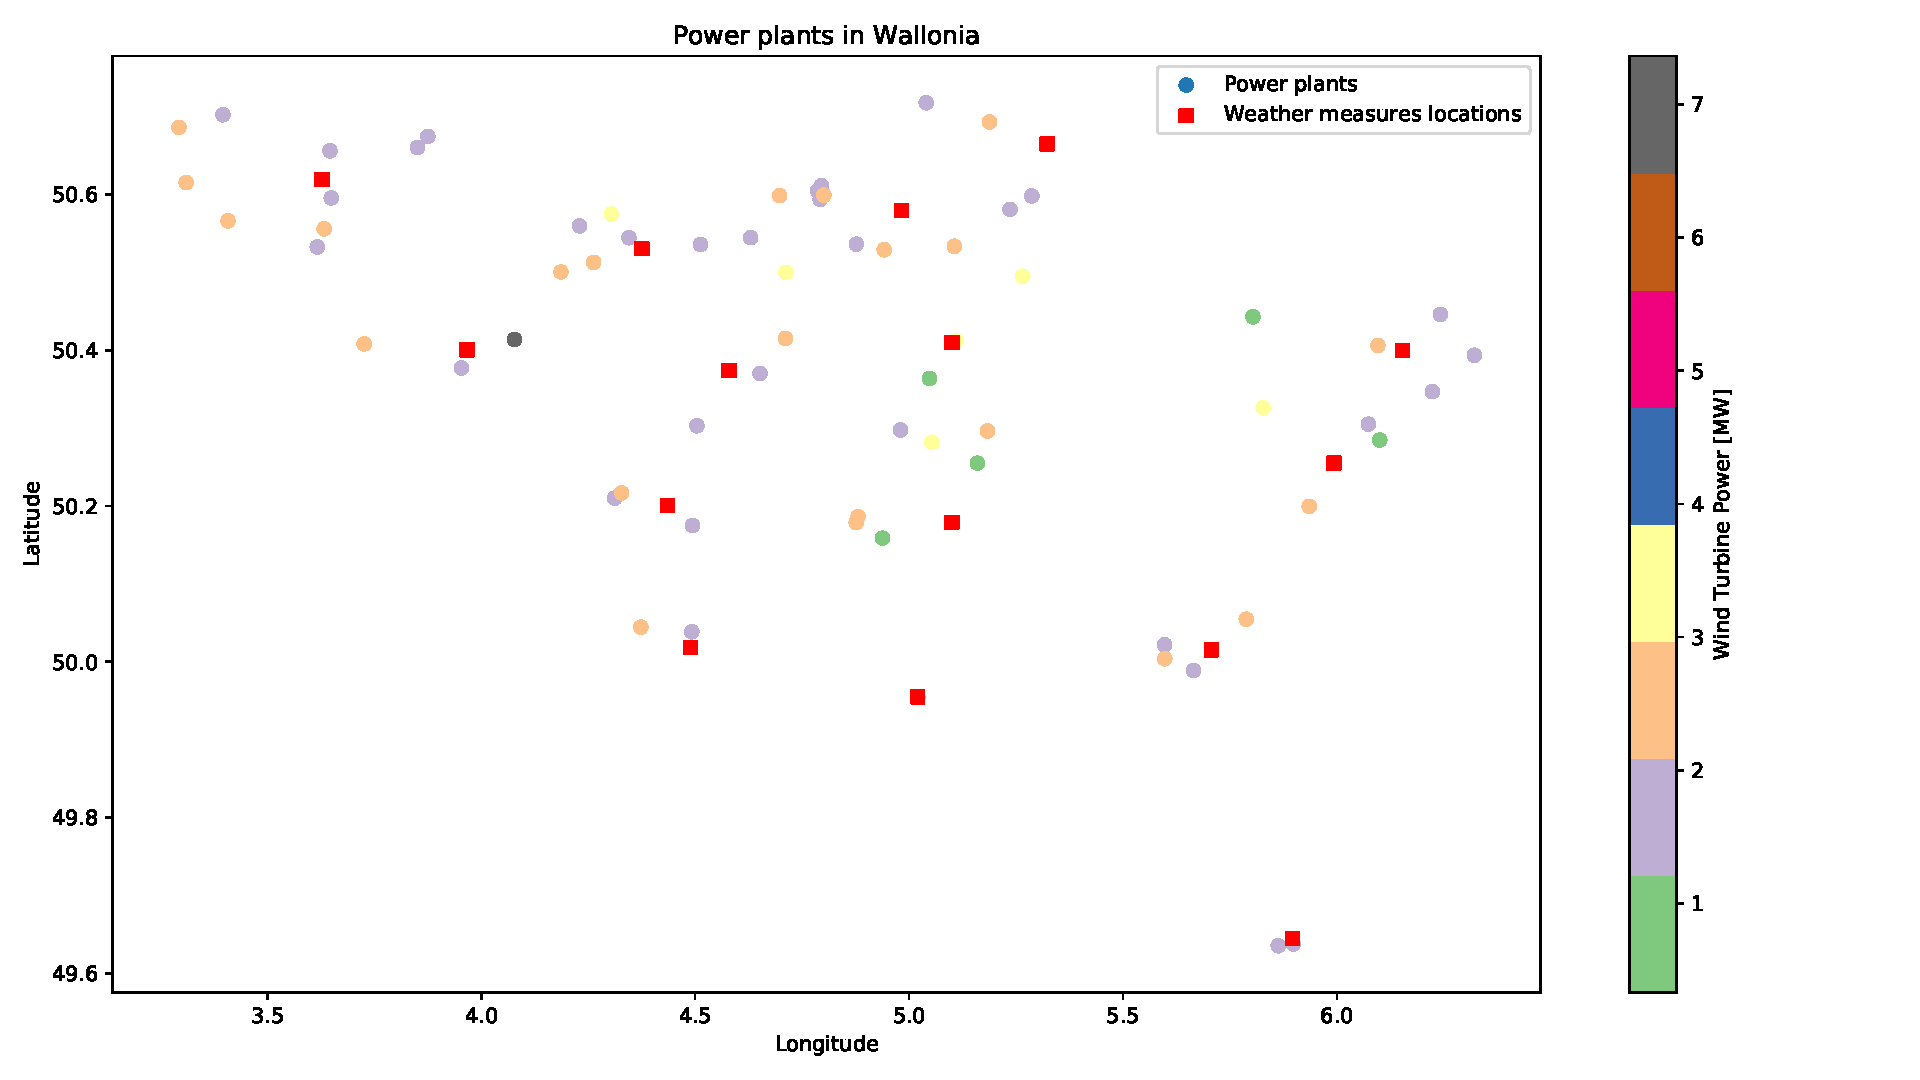
\includegraphics[width=0.6\textwidth]{resources/pdf/power_plants.pdf}
        \caption{Power plants and weather measures in Wallonia}
        \label{fig:power_plants}
    \end{figure}
\end{frame}

\begin{frame}{Metrics\footnote{Messner et. al, Evaluation of Wind Power Forecasts – An up-to-date view, 2020 \cite{messner2020windpower}}}
    \begin{itemize}
        \item MAE: Mean Absolute Error
        \item sMAE / nMAE: standardized / normalized Mean Absolute Error
        \item MQL: Mean Quantile Loss\footnote{Meinshausen, Quantile Regression Forests, 2006 \cite{meinshausen2006quantile}}
        $$\alpha(y, q) = \begin{cases}\alpha \abs{y - q} & \text{ if } y > q \\ (1 - \alpha) \abs{y - q} & \text{ if } y \leq q\end{cases}$$
    \end{itemize}
    \begin{center}
        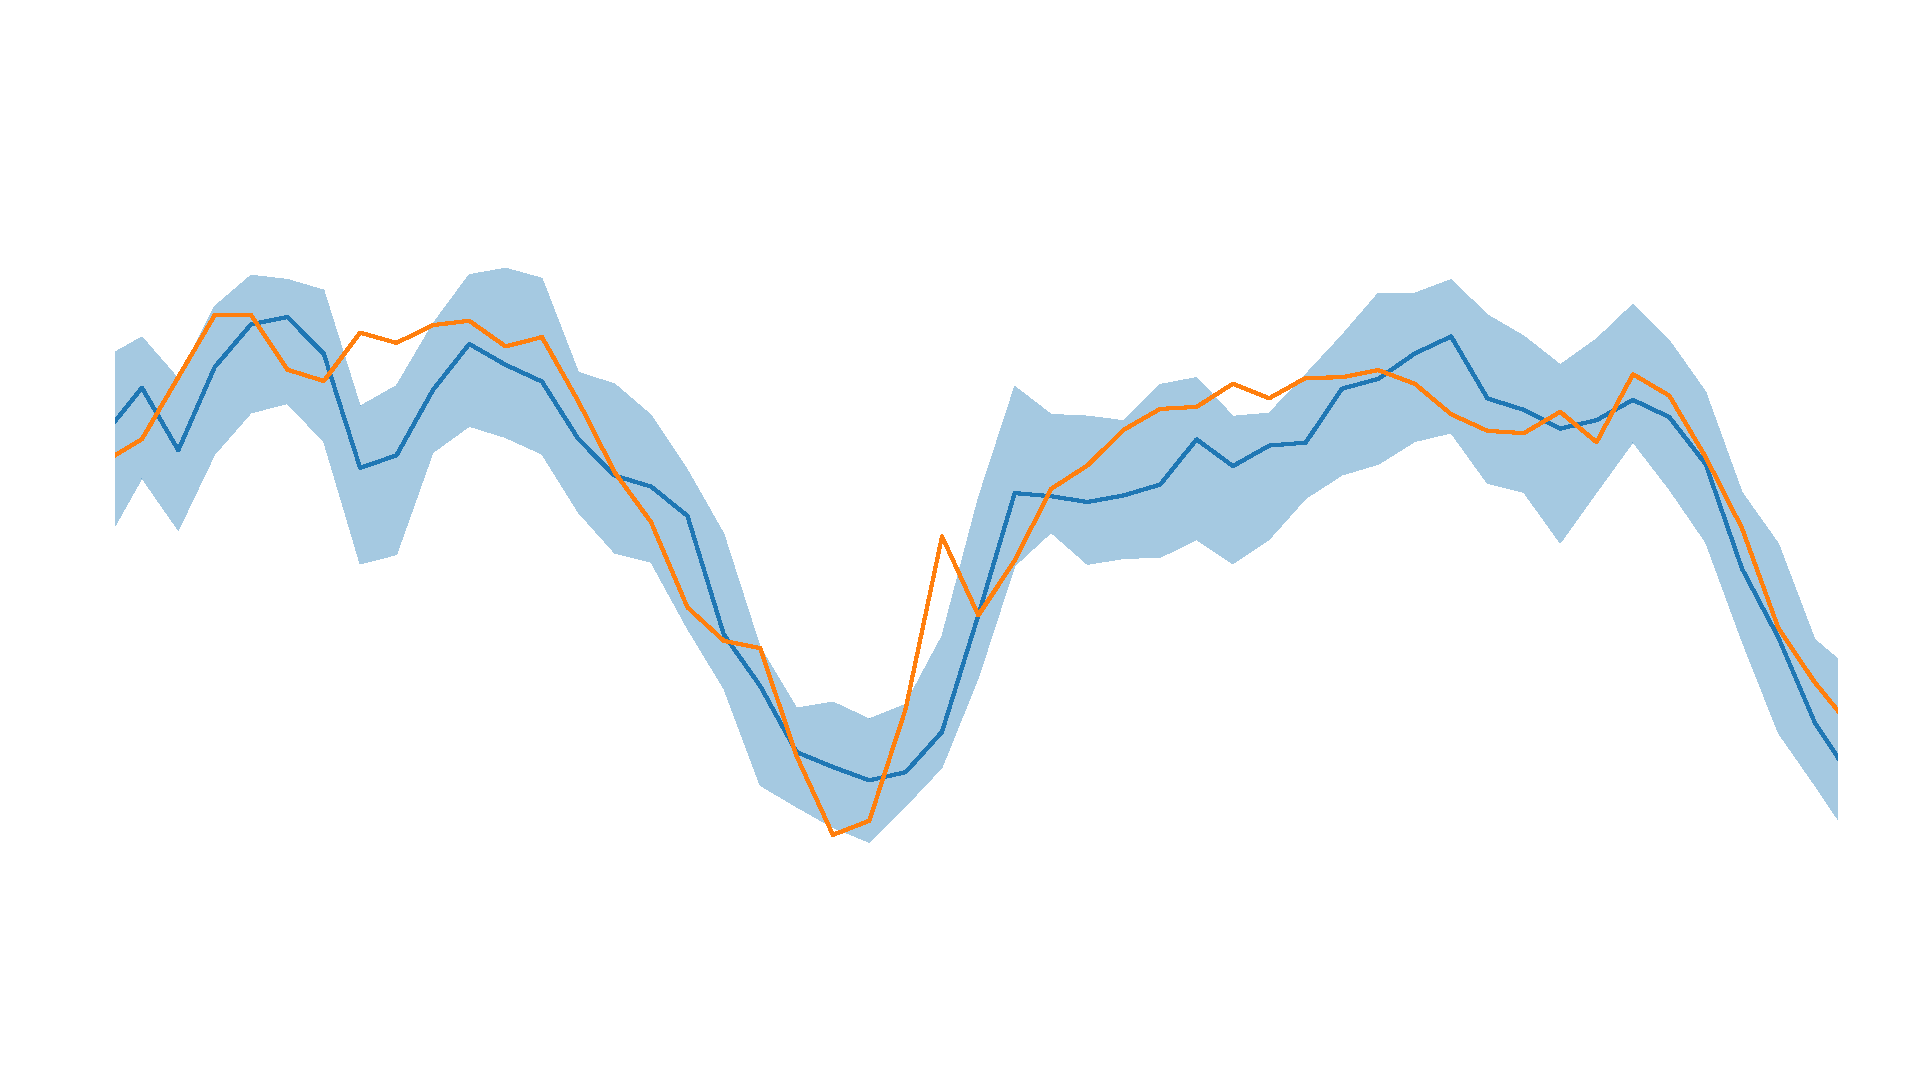
\includegraphics[width=.4\textwidth]{resources/pdf/quantiles.pdf}
    \end{center}
\end{frame}

\begin{frame}{Models: assessment and selection protocols}
    Models:
    \begin{itemize}
        \item Tree bagging method: \alert{Extra Trees}
        \item Tree boosting method: \alert{Gradient Boosting}
    \end{itemize}
    
    Protocols:
    \begin{itemize}
        \item Protocol 1: train on 2019, \alert{test on February 2020}: allows visualizing the prediction
        \item Protocol 2: \num{1.5} year \alert{shuffled} using $30 \times 24$ samples as test set: reduces the bias in the test set.
    \end{itemize}
\end{frame}

\begin{frame}{Results}
    \begin{table}[H]
        \centering
        \begin{tabular}{|c|c|c|}
            \hline 
            MAE & Extra Trees & Gradient Boosting \\ \hline
            Protocol 1 & 36.35 & 36.93 \\ \hline
            Protocol 2 & \uncover<2->{25.37} & \uncover<2->{28.18} \\ \hline
        \end{tabular}
        \noskipcaption{Train set CV scores}
        \label{tab:cv_train}
    \end{table}
\end{frame}

\begin{frame}{Results}
    \begin{table}[H]
        \centering
        \resizebox{\textwidth}{!}{
            \begin{tabular}{|c|c|c|c|c|c|}
                \hline
                Protocol & Method & MAE & sMAE\footnote{To be compared with Croonenbroeck and Dahl, Accurate Medium-Term Wind Power Forecasting in a Censored Classification Framework, 2014 \cite{croonenbroeck2014windpower}} & MQL10 & MQL90 \\ \hline
                \multirow{2}{*}{Protocol 1} &
                Extra Trees &
                42.38 &
                6.00\% &
                \alert{69.86} & % 
                \alert{60.51} \\ \cline{2-6} % 
                 & Gradient Boosting &
                 43.08 &
                 6.10\% &
                 \alert{63.62} & % 
                 \alert{50.94} \\ \hline % 
                \multirow{2}{*}{Protocol 2} &
                \uncover<2->{Extra Trees} &
                \uncover<2->{28.13} &
                \uncover<2->{4.03\%} &
                \uncover<2->{\alert{44.67}} & % 
                \uncover<2->{\alert{51.91}} \\ \cline{2-6} % 
                 & \uncover<2->{Gradient Boosting} &
                 \uncover<2->{31.11} &
                 \uncover<2->{4.46\%} &
                 \uncover<2->{\alert{47.24}} & % 
                 \uncover<2->{\alert{50.24}} \\ \hline % 
            \end{tabular}
        }
        \noskipcaption{Test set scores}
        \label{tab:test_scores}
    \end{table}
\end{frame}

\begin{frame}{Results}
    \begin{figure}
        \centering
        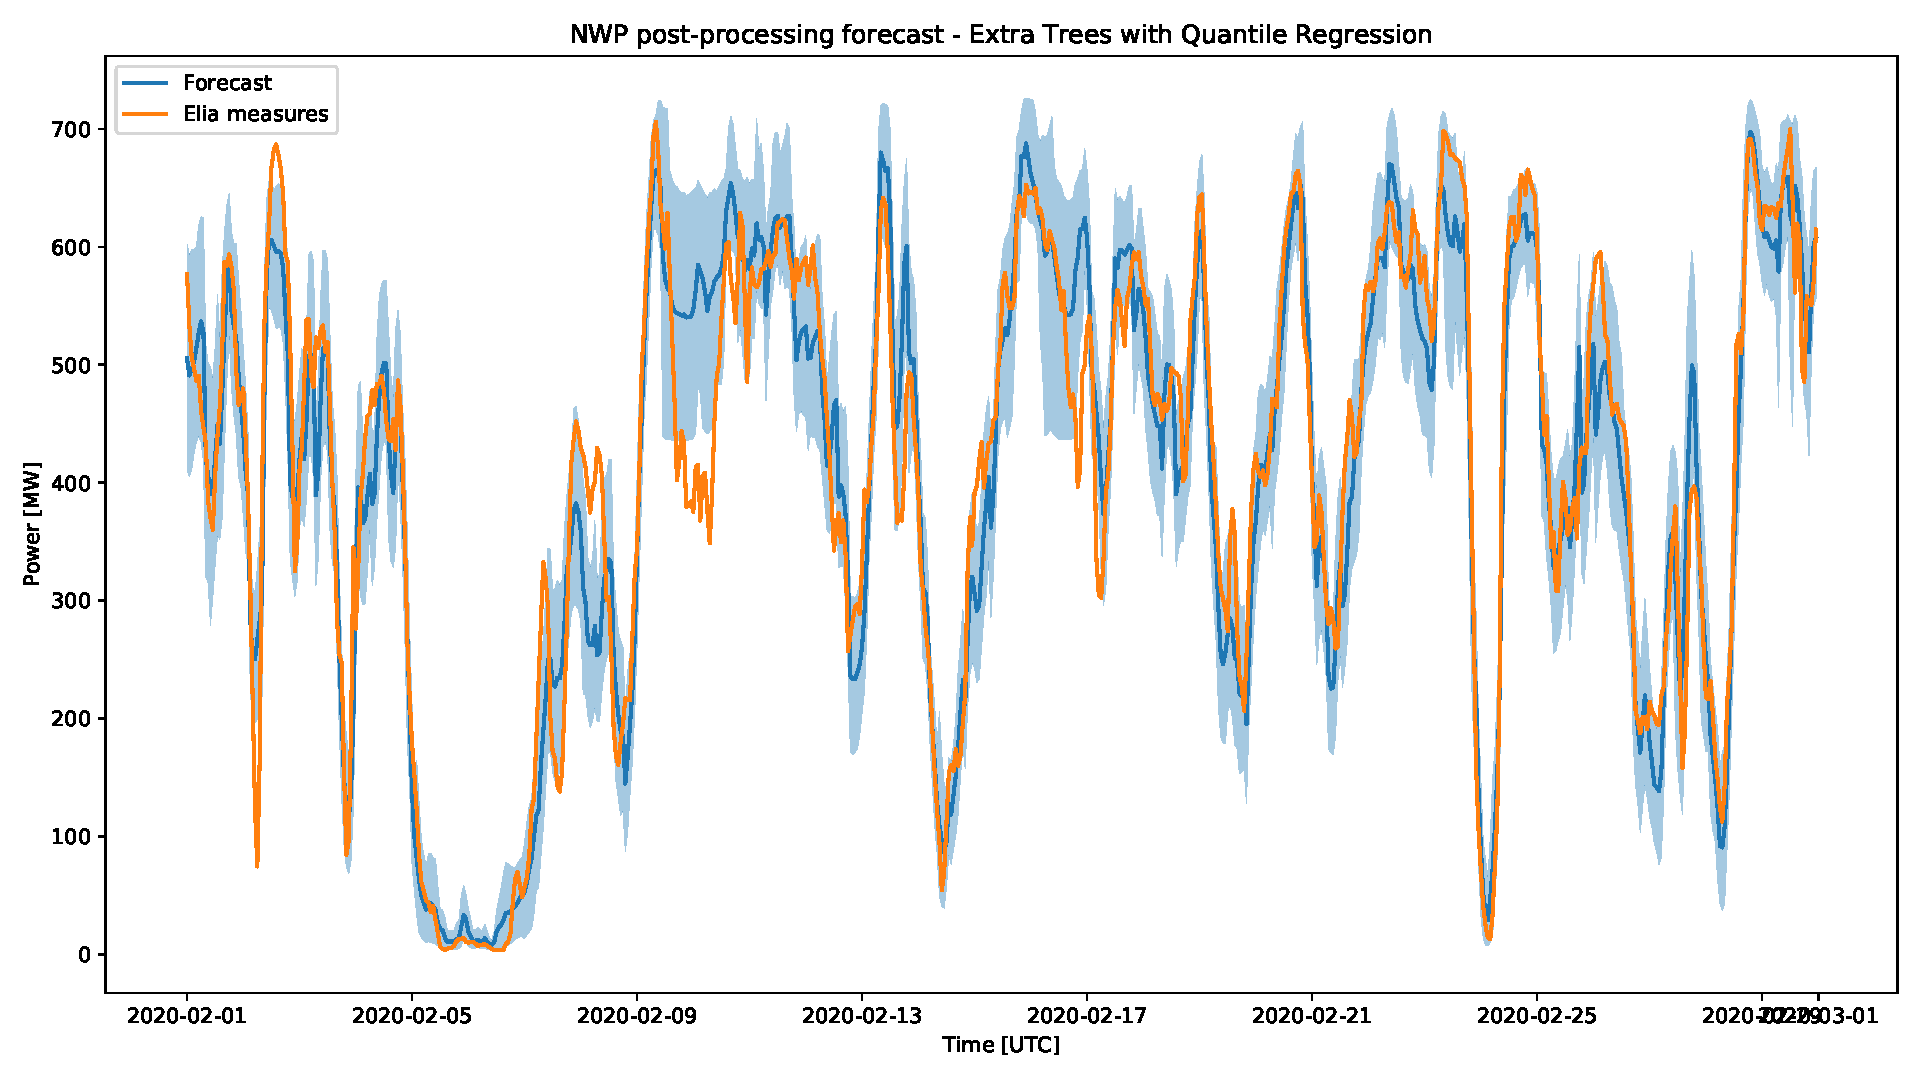
\includegraphics[width=\textwidth]{resources/pdf/extra_trees_p1.pdf}
        \caption{Extra Trees with Quantile Regression - Forecasting for Protocol 1}
        \label{fig:extra_trees}
    \end{figure}
\end{frame}

\begin{frame}{Results}
    \begin{figure}
        \centering
        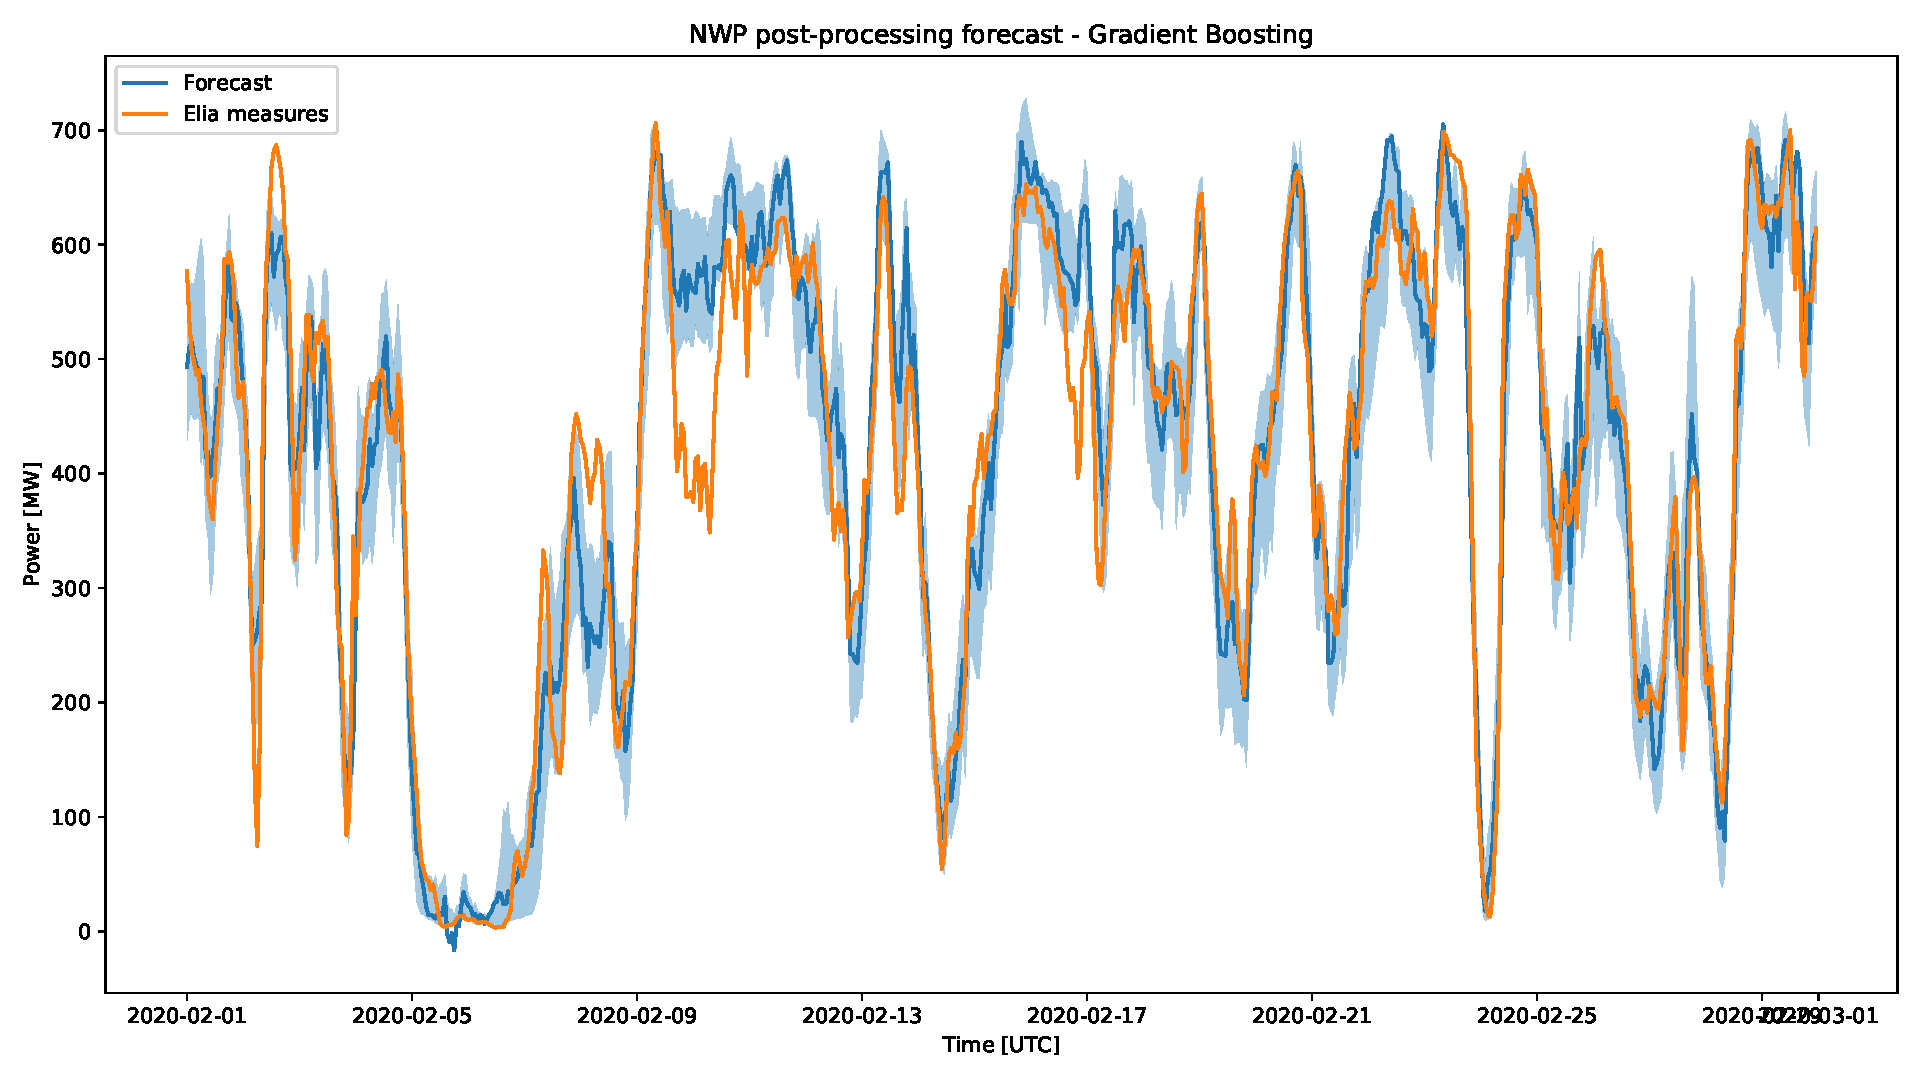
\includegraphics[width=\textwidth]{resources/pdf/gradient_boosting_p1.pdf}
        \caption{Gradient Boosting with Quantile Regression - Forecasting for Protocol 1}
        \label{fig:gradient_boosting}
    \end{figure}
\end{frame}

\begin{frame}{Next objectives}
    \begin{itemize}
        \item Adding 3 new variables in the learning set
        \begin{itemize}
            \item one-day before measurements
            \item total wind power in Wallonia \alert{over time}
            \item total monitored power by Elia \alert{over time}
        \end{itemize}
        \item Testing a MLP as SL learning method
        \item Having a look at feature importances and considering feature selection
        \item Testing and assessing the quality of the forecast on actual weather prediction (NWP) instead of weather measurements
    \end{itemize}
\end{frame}

\begin{frame}[allowframebreaks]
    \printbibliography
\end{frame}

\end{document}
